% *********************************************************************
% © 2016–2023 Jeremy Sylvestre
%
% Permission is granted to copy, distribute and/or modify this document
% under the terms of the GNU Free Documentation License, Version 1.3 or
% any later version published by the Free Software Foundation; with no
% Invariant Sections, no Front-Cover Texts, and no Back-Cover Texts. A
% copy of the license is included in the appendix entitled “GNU Free
% Documentation License” that appears in the output document of this
% PreTeXt source code. All trademarks™ are the registered® marks of
% their respective owners.
%
% *********************************************************************
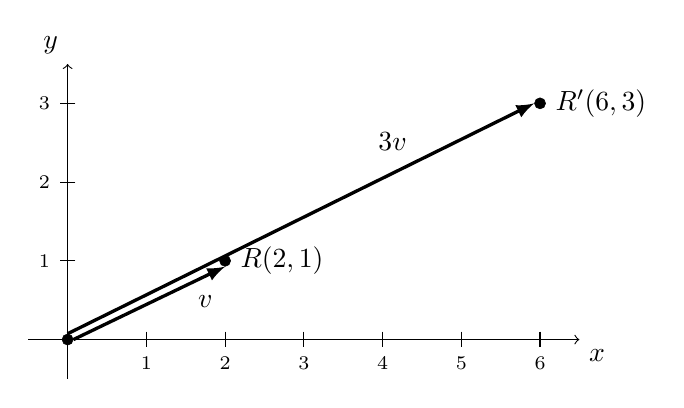
\begin{tikzpicture}[
	point/.style={circle,draw,very thin,fill,inner sep=0pt,minimum size=4pt},
	vector/.style={-latex},
]

	% 3x
%	\begin{scope}
		\draw[->] (-0.5,0) to (6.5,0) node[below right] {$x$};
		\draw[->] (0,-0.5) to (0,3.5) node[above left] {$y$};
		\foreach \x in {1,2,3,4,5,6} {
			\draw (\x,0.1) to (\x,-0.1) node[below] {$\scriptstyle \x$};
		}
		\foreach \y in {1,2,3} {
			\draw (0.1,\y) to (-0.1,\y) node[left] {$\scriptstyle \y$};
		}
		\node[point] at (0,0) (o) {};
		\node[point] at (2,1) (r) [label=right:{$R(2,1)$}] {};
		\node[point] at (6,3) (r2) [label=right:{$R'(6,3)$}] {};
		\draw[vector,very thick] (o.north) to node[above left,near end] {$3\uvec{v}$} (r2.west);
		\draw[vector,very thick] (o.east) to node[below right,near end] {$\uvec{v}$} (r.south);
%	\end{scope}

\end{tikzpicture}
